%%%%%%%%%%%%%%%%%%%%%%%%%%%%%%%%%%%%%%%%%%%%%%%%
% 1. Document class 
\documentclass[a4paper,12pt]{article} % This defines the style of your paper
%%%%%%%%%%%%%%%%%%%%%%%%%%%%%%%%%%%%%%%%%%%%%%%%
% 2. Packages
\usepackage[top = 2.5cm, bottom = 2.5cm, left = 2.5cm, right = 2.5cm]{geometry} 
\usepackage[T1]{fontenc}
\usepackage[utf8]{inputenc}
\usepackage{multirow} % Multirow is for tables with multiple rows within one cell.
\usepackage{booktabs} % For even nicer tables.
\usepackage{graphicx} 
\usepackage{setspace}
\setlength{\parindent}{0in}
\usepackage{float}
\usepackage{fancyhdr}
\usepackage{titlesec}
\usepackage{url}
\usepackage{amsmath,amssymb,amsthm,bm}
\usepackage{subcaption}

\titleformat*{\section}{\large\bfseries}
\titleformat*{\subsection}{\bfseries}
%%%%%%%%%%%%%%%%%%%%%%%%%%%%%%%%%%%%%%%%%%%%%%%%
% 3. Header (and Footer)
\pagestyle{fancy} % With this command we can customize the header style.
\fancyhf{} % This makes sure we do not have other information in our header or footer.
\lhead{\footnotesize  CS 7180}% \lhead puts text in the top left corner. \footnotesize sets our font to a smaller size.
%\rhead works just like \lhead (you can also use \chead)
\rhead{\footnotesize Assignment 1} %<---- Fill in your lastnames.
% Similar commands work for the footer (\lfoot, \cfoot and \rfoot).
% We want to put our page number in the center.
\cfoot{\footnotesize \thepage}

\graphicspath{ {imgs/} }

\begin{document}
\thispagestyle{empty} % This command disables the header on the first page. 

\begin{tabular}{p{15.5cm}} % This is a simple tabular environment to align your text nicely 
{\large \bf CS 7180 Special Topics in AI: Deep Learning} \\
Northeastern University, Spring 2019 \\
\hline % \hline produces horizontal lines.
\end{tabular} % Our tabular environment ends here.

\vspace*{0.3cm} % Now we want to add some vertical space in between the line and our title.

\begin{center} % Everything within the center environment is centered.
    {\Large \bf Assignment 1} % <---- Don't forget to put in the right number
    \vspace{2mm}
    
        % YOUR NAMES GO HERE
    {Name: Tyler Brown UID: 001684955}
\end{center} 
%
\vspace{0.2cm}

\section{Problem 1}

Assignment 1 requested that we use PyTorch to build a CNN to classify
handwritten digits from the MNIST dataset. We were then asked to explore
regularization methodologies such as BatchNorm, Dropout, and L2. The
hyperparameters in Table \ref{table:hyperparams} were used on all models
trained for 10 epochs.

\begin{table}[ht]
\centering
\caption{MNIST CNN Model Hyperparameters}
\label{table:hyperparams}
\begin{tabular}[t]{ll}
\toprule
&Value\\
\midrule
Batch Size & 32 \\
Test Batch Size & 1000 \\
Epochs & 10 \\
Learning Rate & 0.001 \\
Momentum & 0.9 \\
Random Seed & 42 \\
\bottomrule
\end{tabular}
\end{table}

The total number of parameters used by the CNN model I constructed is
643,755 which is less than the maximum number of 1 million parameters. My
CNN model is constructed as follows:
\[
\boxed{\text{Conv layer 1}} \rightarrow
\boxed{\text{Conv layer 2}} \rightarrow
\boxed{\text{Dropout}} \rightarrow
\boxed{\text{Fully Connected 1}}\rightarrow
\underset{output}{\boxed{\text{Fully Connected 2}}}
\]

Categorical cross entropy is used as the loss function. Stochastic
Gradient Descent (SGD) is used for optimization. Each Conv layer
contained a $Conv2d$ layer, ReLU activation function, and
$MaxPool2d$ layer with a kernel size and stride of 2. My approach is
informed by reviewing several implementations of this problem and adopting
a similar framework but with modifications for different forms of
regularization, and batch normalization. Conv layer 2 includes a
$BatchNorm2d$ layer with 75 features. The assignment requested Batch
Normalization to be included in the model so I added it but did not
experiment too much because my implementation was already above the
$0.985$ test accuracy threshold. The Dropout layer was excluded, $p=0.0$,
except when specifically requested by this assignment. \linebreak

\begin{table}[ht]
\centering
\caption{Test Results after 1 Epoch with Dropout, CNN, BatchNorm}
\label{table:dropout}
\begin{tabular}[t]{lcr}
\toprule
&Average Loss & Accuracy\\
$p=0.0$ & 2.3494 & 6.22\% \\
$p=0.1$ & 2.3512 & 11.69\%\\
$p=0.2$ & 2.3517 & 12.20\%\\
$p=0.3$ & 2.3255 & 8.72\% \\
$p=0.4$ & 2.3080 & 12.37\%\\
$p=0.5$ & 2.3446 & 10.64\%\\
$p=0.6$ & 2.3429 & 9.00\%\\
$p=0.7$ & 2.2936 & 12.68\%\\
$p=0.8$ & 2.3343 & 10.30\%\\
$p=0.9$ & 2.3098 & 7.69\%\\
$p=1.0$ & 2.3137 & 10.13\%\\
\midrule
\bottomrule
\end{tabular}
\end{table}


Table \ref{table:dropout} contains results from using a range of probabilities
between 0 and 1. The test results after 1 epoch show that varying levels
of dropout didn't allow for more than 0.15 accuracy, far below 0.985. I've
read that dropout usually hurts perfomance at the beginning of training but
provides improvements when the model is closer to convergence. Therefore,
judging dropout performance after 1 epoch should be problematic.\newline

Results from Table \ref{table:results} show how dropout is still associated
with poor performance in this use case even after training for 10 epochs.
I have seen other implementations of CNN use dropout with reasonable
results so I'm open to the possibility of getting good results from dropout
with alternative model specifications. \newline

\begin{table}[ht]
\centering
\caption{Test Results after 10 Epochs}
\label{table:results}
\begin{tabular}[t]{lcc} 
\toprule
&Average Loss & Accuracy\\
\midrule
CNN,BatchNorm               & 0.0261 & 99.17\% \\
CNN,BatchNorm, Dropout=0.25 & 2.3230 & 10.06\% \\
CNN,BatchNorm, L2=0.002     & 0.0340 & 98.95\% \\
\bottomrule
\end{tabular}
\end{table}

We can see that a CNN model without L2 regularization outperforms the
other models. However, when we review Figure \ref{fig:cnn} containing
\textit{Loss vs. Epochs} and \textit{Accuracy vs. Epochs} it becomes
clear that the training set is overfitting relative to the development/test
set. 

\begin{figure}[h]
  \centering
  \caption{CNN with Batch Norm}
  \label{fig:cnn}
  \begin{subfigure}[h]{0.45\textwidth}
    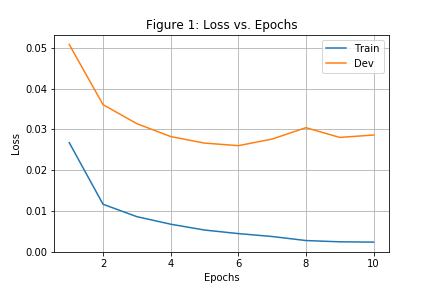
\includegraphics[width=\textwidth]{fig1}
  \end{subfigure}
  \begin{subfigure}[h]{0.45\textwidth}
    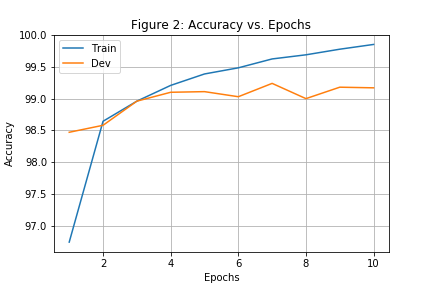
\includegraphics[width=\textwidth]{fig2}
  \end{subfigure}
\end{figure}

We need to consider strategies to address overfitting in Figure \ref{fig:cnn}
or the model should not generalize well in theory, even though the accuracy
score is slightly higher for the development set. We cannot add data in this
exercise so it's important to consider other regularization strategies to
increase bias to reduce overfitting. Figure \ref{fig:cnnL2} shows what happens
when L2 regularization is used. The accuracy results across epochs in
Figure \ref{fig:cnnL2} show the development set tracking much more closely
with the training set than we saw in Figure \ref{fig:cnn}. It's possible that
L2 regularization may benefit from early stopping after 8 epochs. This
seems to be when the training set and development have accuracy scores
that converge and reach their maximum. \newline


\begin{figure}[t]
  \caption{CNN with Batch Norm and L2 Regularization=0.002}
  \label{fig:cnnL2}
  \begin{subfigure}{0.45\textwidth}
    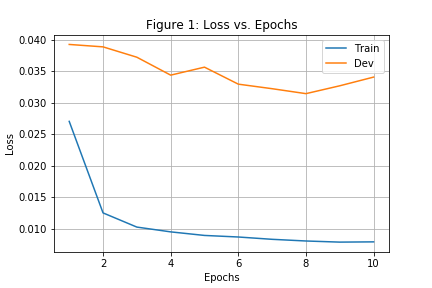
\includegraphics[width=\textwidth]{fig3}
  \end{subfigure}
  \begin{subfigure}{0.45\textwidth}
    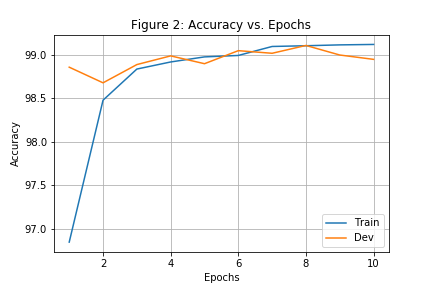
\includegraphics[width=\textwidth]{fig4}
  \end{subfigure}
\end{figure}

The most effective strategies I found for increasing accuracy using a
CNN, given a well accepted model specification, is increasing the number
of neurons in a layer while tuning L2 regularization to prevent overfitting.
In future iterations, I would explore techniques such as early stopping and
randomized selection of hyperparameters such as learning rate. In past
models, I've found learning rate to be a hyperparameter which is very
meaningful for performance. This homework has helped me get exposure to
Pytorch and AWS Sagemaker.

\end{document}
